\documentclass[12pt]{report}

\usepackage{amsmath} % loads AMS-Math package
\usepackage{euscript}
\usepackage{amssymb}
\usepackage{epsfig} % allows PostScript files
\usepackage{graphicx}
\usepackage{multirow}
\usepackage{listings} % allows lstlisting environment
\usepackage{moreverb} % allows listinginput environment
\usepackage{vmargin} % allows better margins
\usepackage{color}
\usepackage{mcode}
\setpapersize{USletter} % sets the paper size
\allowdisplaybreaks[1]
\setmarginsrb{1in}{0.7in}{1in}{1in}{12pt}{11mm}{0pt}{11mm} %sets margins


\title{\LaTeX \ Title }

\author{Alex Beutel  \\
{\small\em \copyright \  Draft date \today }}

 \date{ }

\begin{document}

\maketitle
\begin{abstract}
	blah blah blah
\end{abstract}
 %\addcontentsline{toc}{chapter}{Contents}
\pagenumbering{roman}
\tableofcontents
\listoffigures
\listoftables

\pagestyle{headings}
\pagenumbering{arabic}

\pagestyle{plain}

\chapter{Introduction}

\input{writing/intro}

\chapter{Chaos Theory}

\section{Nonlinear Dynamics}
\label{sec: Nonlinear Dynamics}
\input{writing/nonlinearDynamics}

\section{Chaos ``Proof"}
\label{sec: Chaos ``Proof"}
\input{writing/chaosProof}

\section{Nonlinear Methods}
\label{sec: Nonlinear Methods}
\input{writing/nonlinearMethods}

\section{Feigenbaum Ratios}
\label{sec: Feigenbaum Ratios}
\input{writing/feigenbaumRatios}

\chapter{Experimental Setup}

\section{RL Diode Circuit}
\label{sec:RL Diode Circuit}
\input{writing/RLDiodeCircuit}

\section{Picoscope}
\label{sec:Picoscope}
\input{writing/picoscope}

\section{Oscilloscope}
\label{sec:Oscilloscope}
\input{writing/oscilloscope}

\chapter{Experimental Procedure}
\input{writing/experimentalProcedure}

	\begin{figure}
		\centering
		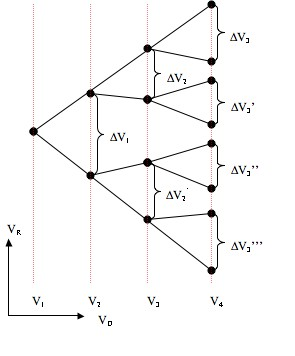
\includegraphics{Pics/BifurcationDiagram.jpg}
		\caption{Calculating Feigenbaum ratios}
		\label{fig: Calculating Feigenbaum ratios}
	\end{figure}
\chapter{Results}

\section{Data Analysis} % (fold)
\label{sec:Data Analysis}

	\begin{figure}[h]
		\centering
		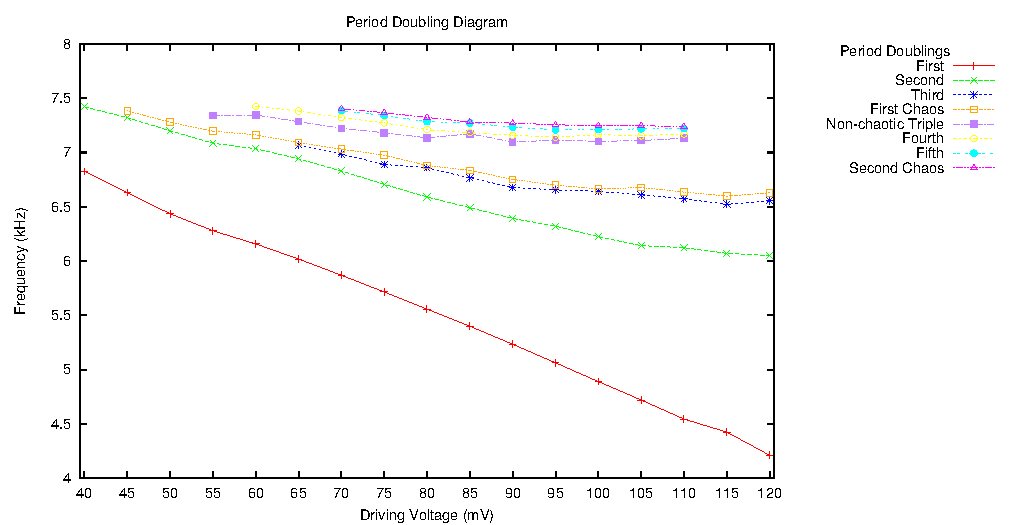
\includegraphics{plots/general.pdf}
		\caption{Period Doubling}
		\label{fig:periodDoubling}
	\end{figure}

\input{writing/periodDoubling}

	\begin{figure}[h]
		\centering
		% GNUPLOT: LaTeX picture
\setlength{\unitlength}{0.240900pt}
\ifx\plotpoint\undefined\newsavebox{\plotpoint}\fi
\sbox{\plotpoint}{\rule[-0.200pt]{0.400pt}{0.400pt}}%
\begin{picture}(1500,900)(0,0)
\sbox{\plotpoint}{\rule[-0.200pt]{0.400pt}{0.400pt}}%
\put(191.0,131.0){\rule[-0.200pt]{4.818pt}{0.400pt}}
\put(171,131){\makebox(0,0)[r]{ 60}}
\put(1429.0,131.0){\rule[-0.200pt]{4.818pt}{0.400pt}}
\put(191.0,212.0){\rule[-0.200pt]{4.818pt}{0.400pt}}
\put(171,212){\makebox(0,0)[r]{ 70}}
\put(1429.0,212.0){\rule[-0.200pt]{4.818pt}{0.400pt}}
\put(191.0,293.0){\rule[-0.200pt]{4.818pt}{0.400pt}}
\put(171,293){\makebox(0,0)[r]{ 80}}
\put(1429.0,293.0){\rule[-0.200pt]{4.818pt}{0.400pt}}
\put(191.0,374.0){\rule[-0.200pt]{4.818pt}{0.400pt}}
\put(171,374){\makebox(0,0)[r]{ 90}}
\put(1429.0,374.0){\rule[-0.200pt]{4.818pt}{0.400pt}}
\put(191.0,455.0){\rule[-0.200pt]{4.818pt}{0.400pt}}
\put(171,455){\makebox(0,0)[r]{ 100}}
\put(1429.0,455.0){\rule[-0.200pt]{4.818pt}{0.400pt}}
\put(191.0,535.0){\rule[-0.200pt]{4.818pt}{0.400pt}}
\put(171,535){\makebox(0,0)[r]{ 110}}
\put(1429.0,535.0){\rule[-0.200pt]{4.818pt}{0.400pt}}
\put(191.0,616.0){\rule[-0.200pt]{4.818pt}{0.400pt}}
\put(171,616){\makebox(0,0)[r]{ 120}}
\put(1429.0,616.0){\rule[-0.200pt]{4.818pt}{0.400pt}}
\put(191.0,697.0){\rule[-0.200pt]{4.818pt}{0.400pt}}
\put(171,697){\makebox(0,0)[r]{ 130}}
\put(1429.0,697.0){\rule[-0.200pt]{4.818pt}{0.400pt}}
\put(191.0,778.0){\rule[-0.200pt]{4.818pt}{0.400pt}}
\put(171,778){\makebox(0,0)[r]{ 140}}
\put(1429.0,778.0){\rule[-0.200pt]{4.818pt}{0.400pt}}
\put(191.0,859.0){\rule[-0.200pt]{4.818pt}{0.400pt}}
\put(171,859){\makebox(0,0)[r]{ 150}}
\put(1429.0,859.0){\rule[-0.200pt]{4.818pt}{0.400pt}}
\put(191.0,131.0){\rule[-0.200pt]{0.400pt}{4.818pt}}
\put(191,90){\makebox(0,0){ 12}}
\put(191.0,839.0){\rule[-0.200pt]{0.400pt}{4.818pt}}
\put(401.0,131.0){\rule[-0.200pt]{0.400pt}{4.818pt}}
\put(401,90){\makebox(0,0){ 14}}
\put(401.0,839.0){\rule[-0.200pt]{0.400pt}{4.818pt}}
\put(610.0,131.0){\rule[-0.200pt]{0.400pt}{4.818pt}}
\put(610,90){\makebox(0,0){ 16}}
\put(610.0,839.0){\rule[-0.200pt]{0.400pt}{4.818pt}}
\put(820.0,131.0){\rule[-0.200pt]{0.400pt}{4.818pt}}
\put(820,90){\makebox(0,0){ 18}}
\put(820.0,839.0){\rule[-0.200pt]{0.400pt}{4.818pt}}
\put(1030.0,131.0){\rule[-0.200pt]{0.400pt}{4.818pt}}
\put(1030,90){\makebox(0,0){ 20}}
\put(1030.0,839.0){\rule[-0.200pt]{0.400pt}{4.818pt}}
\put(1239.0,131.0){\rule[-0.200pt]{0.400pt}{4.818pt}}
\put(1239,90){\makebox(0,0){ 22}}
\put(1239.0,839.0){\rule[-0.200pt]{0.400pt}{4.818pt}}
\put(1449.0,131.0){\rule[-0.200pt]{0.400pt}{4.818pt}}
\put(1449,90){\makebox(0,0){ 24}}
\put(1449.0,839.0){\rule[-0.200pt]{0.400pt}{4.818pt}}
\put(191.0,131.0){\rule[-0.200pt]{0.400pt}{175.375pt}}
\put(191.0,131.0){\rule[-0.200pt]{303.052pt}{0.400pt}}
\put(1449.0,131.0){\rule[-0.200pt]{0.400pt}{175.375pt}}
\put(191.0,859.0){\rule[-0.200pt]{303.052pt}{0.400pt}}
\put(50,495){\makebox(0,0){\shortstack{V$_{\rm resistor}$\\(mV)}}}
\put(820,29){\makebox(0,0){V$_{\rm drive}$ (mV)}}
\put(243,159){\rule{1pt}{1pt}}
\put(327,196){\rule{1pt}{1pt}}
\put(359,212){\rule{1pt}{1pt}}
\put(422,228){\rule{1pt}{1pt}}
\put(464,244){\rule{1pt}{1pt}}
\put(537,269){\rule{1pt}{1pt}}
\put(621,297){\rule{1pt}{1pt}}
\put(726,325){\rule{1pt}{1pt}}
\put(747,329){\rule{1pt}{1pt}}
\put(768,353){\rule{1pt}{1pt}}
\put(768,313){\rule{1pt}{1pt}}
\put(799,370){\rule{1pt}{1pt}}
\put(799,301){\rule{1pt}{1pt}}
\put(830,394){\rule{1pt}{1pt}}
\put(830,269){\rule{1pt}{1pt}}
\put(872,406){\rule{1pt}{1pt}}
\put(872,252){\rule{1pt}{1pt}}
\put(914,426){\rule{1pt}{1pt}}
\put(914,236){\rule{1pt}{1pt}}
\put(956,455){\rule{1pt}{1pt}}
\put(956,216){\rule{1pt}{1pt}}
\put(1019,499){\rule{1pt}{1pt}}
\put(1019,208){\rule{1pt}{1pt}}
\put(1103,224){\rule{1pt}{1pt}}
\put(1103,552){\rule{1pt}{1pt}}
\put(1145,576){\rule{1pt}{1pt}}
\put(1145,232){\rule{1pt}{1pt}}
\put(1155,592){\rule{1pt}{1pt}}
\put(1155,568){\rule{1pt}{1pt}}
\put(1155,264){\rule{1pt}{1pt}}
\put(1155,216){\rule{1pt}{1pt}}
\put(1166,608){\rule{1pt}{1pt}}
\put(1166,556){\rule{1pt}{1pt}}
\put(1166,236){\rule{1pt}{1pt}}
\put(1166,252){\rule{1pt}{1pt}}
\put(1176,620){\rule{1pt}{1pt}}
\put(1176,552){\rule{1pt}{1pt}}
\put(1176,273){\rule{1pt}{1pt}}
\put(1176,240){\rule{1pt}{1pt}}
\put(1187,624){\rule{1pt}{1pt}}
\put(1187,552){\rule{1pt}{1pt}}
\put(1187,244){\rule{1pt}{1pt}}
\put(1187,285){\rule{1pt}{1pt}}
\put(1197,633){\rule{1pt}{1pt}}
\put(1197,620){\rule{1pt}{1pt}}
\put(1197,572){\rule{1pt}{1pt}}
\put(1197,552){\rule{1pt}{1pt}}
\put(1197,293){\rule{1pt}{1pt}}
\put(1197,285){\rule{1pt}{1pt}}
\put(1197,236){\rule{1pt}{1pt}}
\put(1197,240){\rule{1pt}{1pt}}
\put(1271,264){\rule{1pt}{1pt}}
\put(1271,301){\rule{1pt}{1pt}}
\put(1271,754){\rule{1pt}{1pt}}
\put(1292,273){\rule{1pt}{1pt}}
\put(1292,305){\rule{1pt}{1pt}}
\put(1292,778){\rule{1pt}{1pt}}
\put(1302,313){\rule{1pt}{1pt}}
\put(1302,232){\rule{1pt}{1pt}}
\put(1302,301){\rule{1pt}{1pt}}
\put(1302,321){\rule{1pt}{1pt}}
\put(1302,786){\rule{1pt}{1pt}}
\put(1302,762){\rule{1pt}{1pt}}
\put(191.0,131.0){\rule[-0.200pt]{0.400pt}{175.375pt}}
\put(191.0,131.0){\rule[-0.200pt]{303.052pt}{0.400pt}}
\put(1449.0,131.0){\rule[-0.200pt]{0.400pt}{175.375pt}}
\put(191.0,859.0){\rule[-0.200pt]{303.052pt}{0.400pt}}
\end{picture}

		\caption{80 kHz Bifurcation plot. $V_{\rm drive}$ error: 0.1 V. $V_{\rm R}$ error: 5 mV.}
		\label{fig:80khzBifurcation}
	\end{figure}

	\begin{figure}[h]
		\centering
		% GNUPLOT: LaTeX picture
\setlength{\unitlength}{0.240900pt}
\ifx\plotpoint\undefined\newsavebox{\plotpoint}\fi
\sbox{\plotpoint}{\rule[-0.200pt]{0.400pt}{0.400pt}}%
\begin{picture}(1500,900)(0,0)
\sbox{\plotpoint}{\rule[-0.200pt]{0.400pt}{0.400pt}}%
\put(191.0,131.0){\rule[-0.200pt]{4.818pt}{0.400pt}}
\put(171,131){\makebox(0,0)[r]{ 50}}
\put(1429.0,131.0){\rule[-0.200pt]{4.818pt}{0.400pt}}
\put(191.0,235.0){\rule[-0.200pt]{4.818pt}{0.400pt}}
\put(171,235){\makebox(0,0)[r]{ 60}}
\put(1429.0,235.0){\rule[-0.200pt]{4.818pt}{0.400pt}}
\put(191.0,339.0){\rule[-0.200pt]{4.818pt}{0.400pt}}
\put(171,339){\makebox(0,0)[r]{ 70}}
\put(1429.0,339.0){\rule[-0.200pt]{4.818pt}{0.400pt}}
\put(191.0,443.0){\rule[-0.200pt]{4.818pt}{0.400pt}}
\put(171,443){\makebox(0,0)[r]{ 80}}
\put(1429.0,443.0){\rule[-0.200pt]{4.818pt}{0.400pt}}
\put(191.0,547.0){\rule[-0.200pt]{4.818pt}{0.400pt}}
\put(171,547){\makebox(0,0)[r]{ 90}}
\put(1429.0,547.0){\rule[-0.200pt]{4.818pt}{0.400pt}}
\put(191.0,651.0){\rule[-0.200pt]{4.818pt}{0.400pt}}
\put(171,651){\makebox(0,0)[r]{ 100}}
\put(1429.0,651.0){\rule[-0.200pt]{4.818pt}{0.400pt}}
\put(191.0,755.0){\rule[-0.200pt]{4.818pt}{0.400pt}}
\put(171,755){\makebox(0,0)[r]{ 110}}
\put(1429.0,755.0){\rule[-0.200pt]{4.818pt}{0.400pt}}
\put(191.0,859.0){\rule[-0.200pt]{4.818pt}{0.400pt}}
\put(171,859){\makebox(0,0)[r]{ 120}}
\put(1429.0,859.0){\rule[-0.200pt]{4.818pt}{0.400pt}}
\put(191.0,131.0){\rule[-0.200pt]{0.400pt}{4.818pt}}
\put(191,90){\makebox(0,0){ 14}}
\put(191.0,839.0){\rule[-0.200pt]{0.400pt}{4.818pt}}
\put(331.0,131.0){\rule[-0.200pt]{0.400pt}{4.818pt}}
\put(331,90){\makebox(0,0){ 15}}
\put(331.0,839.0){\rule[-0.200pt]{0.400pt}{4.818pt}}
\put(471.0,131.0){\rule[-0.200pt]{0.400pt}{4.818pt}}
\put(471,90){\makebox(0,0){ 16}}
\put(471.0,839.0){\rule[-0.200pt]{0.400pt}{4.818pt}}
\put(610.0,131.0){\rule[-0.200pt]{0.400pt}{4.818pt}}
\put(610,90){\makebox(0,0){ 17}}
\put(610.0,839.0){\rule[-0.200pt]{0.400pt}{4.818pt}}
\put(750.0,131.0){\rule[-0.200pt]{0.400pt}{4.818pt}}
\put(750,90){\makebox(0,0){ 18}}
\put(750.0,839.0){\rule[-0.200pt]{0.400pt}{4.818pt}}
\put(890.0,131.0){\rule[-0.200pt]{0.400pt}{4.818pt}}
\put(890,90){\makebox(0,0){ 19}}
\put(890.0,839.0){\rule[-0.200pt]{0.400pt}{4.818pt}}
\put(1030.0,131.0){\rule[-0.200pt]{0.400pt}{4.818pt}}
\put(1030,90){\makebox(0,0){ 20}}
\put(1030.0,839.0){\rule[-0.200pt]{0.400pt}{4.818pt}}
\put(1169.0,131.0){\rule[-0.200pt]{0.400pt}{4.818pt}}
\put(1169,90){\makebox(0,0){ 21}}
\put(1169.0,839.0){\rule[-0.200pt]{0.400pt}{4.818pt}}
\put(1309.0,131.0){\rule[-0.200pt]{0.400pt}{4.818pt}}
\put(1309,90){\makebox(0,0){ 22}}
\put(1309.0,839.0){\rule[-0.200pt]{0.400pt}{4.818pt}}
\put(1449.0,131.0){\rule[-0.200pt]{0.400pt}{4.818pt}}
\put(1449,90){\makebox(0,0){ 23}}
\put(1449.0,839.0){\rule[-0.200pt]{0.400pt}{4.818pt}}
\put(191.0,131.0){\rule[-0.200pt]{0.400pt}{175.375pt}}
\put(191.0,131.0){\rule[-0.200pt]{303.052pt}{0.400pt}}
\put(1449.0,131.0){\rule[-0.200pt]{0.400pt}{175.375pt}}
\put(191.0,859.0){\rule[-0.200pt]{303.052pt}{0.400pt}}
\put(50,495){\makebox(0,0){\shortstack{V$_{\rm R}$\\(mV)}}}
\put(820,29){\makebox(0,0){V$_{\rm drive}$ (mV)}}
\put(261,188){\rule{1pt}{1pt}}
\put(317,214){\rule{1pt}{1pt}}
\put(373,225){\rule{1pt}{1pt}}
\put(429,251){\rule{1pt}{1pt}}
\put(429,204){\rule{1pt}{1pt}}
\put(485,282){\rule{1pt}{1pt}}
\put(485,183){\rule{1pt}{1pt}}
\put(568,323){\rule{1pt}{1pt}}
\put(568,157){\rule{1pt}{1pt}}
\put(624,349){\rule{1pt}{1pt}}
\put(624,147){\rule{1pt}{1pt}}
\put(680,375){\rule{1pt}{1pt}}
\put(680,136){\rule{1pt}{1pt}}
\put(764,412){\rule{1pt}{1pt}}
\put(764,136){\rule{1pt}{1pt}}
\put(848,136){\rule{1pt}{1pt}}
\put(848,443){\rule{1pt}{1pt}}
\put(960,500){\rule{1pt}{1pt}}
\put(960,173){\rule{1pt}{1pt}}
\put(1016,511){\rule{1pt}{1pt}}
\put(1016,178){\rule{1pt}{1pt}}
\put(1072,531){\rule{1pt}{1pt}}
\put(1072,505){\rule{1pt}{1pt}}
\put(1072,173){\rule{1pt}{1pt}}
\put(1072,188){\rule{1pt}{1pt}}
\put(1100,547){\rule{1pt}{1pt}}
\put(1100,511){\rule{1pt}{1pt}}
\put(1100,225){\rule{1pt}{1pt}}
\put(1100,178){\rule{1pt}{1pt}}
\put(1141,573){\rule{1pt}{1pt}}
\put(1141,511){\rule{1pt}{1pt}}
\put(1141,204){\rule{1pt}{1pt}}
\put(1141,245){\rule{1pt}{1pt}}
\put(1183,578){\rule{1pt}{1pt}}
\put(1183,563){\rule{1pt}{1pt}}
\put(1183,531){\rule{1pt}{1pt}}
\put(1183,500){\rule{1pt}{1pt}}
\put(1183,277){\rule{1pt}{1pt}}
\put(1183,245){\rule{1pt}{1pt}}
\put(1183,199){\rule{1pt}{1pt}}
\put(1183,188){\rule{1pt}{1pt}}
\put(1323,245){\rule{1pt}{1pt}}
\put(1323,407){\rule{1pt}{1pt}}
\put(1323,599){\rule{1pt}{1pt}}
\put(1351,755){\rule{1pt}{1pt}}
\put(1351,739){\rule{1pt}{1pt}}
\put(1351,277){\rule{1pt}{1pt}}
\put(1351,297){\rule{1pt}{1pt}}
\put(1351,287){\rule{1pt}{1pt}}
\put(1351,204){\rule{1pt}{1pt}}
\put(191.0,131.0){\rule[-0.200pt]{0.400pt}{175.375pt}}
\put(191.0,131.0){\rule[-0.200pt]{303.052pt}{0.400pt}}
\put(1449.0,131.0){\rule[-0.200pt]{0.400pt}{175.375pt}}
\put(191.0,859.0){\rule[-0.200pt]{303.052pt}{0.400pt}}
\end{picture}

		\caption{100 kHz Bifurcation plot. $V_{\rm drive}$ error: 0.1 V. $V_{\rm R}$ error: 5 mV.}
		\label{fig:100khzBifurcation}
	\end{figure}
	
\input{writing/bifurcationPlots}
	
	\begin{table}
		\centering
		\begin{tabular}{|c|c|c|c|c|}
			\hline
			Test & $\bar\delta$ & $\sigma_{\bar\delta}$ & $\bar\alpha$ & $\sigma_{\bar\alpha}$                 \\ \hline
\multirow{4}{*}{80 kHz} & 4.866354752 & 0.587017407 & 5.00952381 & 5.677672139        \\\cline{2-5} 
 & 5.071945093 & 3.588190355 & 5.96026196 & 7.723440964              \\ \cline{2-5} 
 &  &  & 31 & 151.037876                                             \\ \cline{2-5} 
 &  &  & 8.818145743 & 14.47253609                                   \\ \hline\hline
 \multirow{4}{*}{120 kHz} & 3.970268152 & 0.233369321 & 7.617629429 & 20.52787139      \\ \cline{2-5} 
 & 6.332809588 & 3.635471291 & 9.867676768 & 31.02307017             \\ \cline{2-5} 
 &  &  & 26.12619048 & 247.3949034                                   \\ \cline{2-5} 
 &  &  & 7.404079254 & 14.37760074                                   \\ \hline \hline
10.444 V & 4.664396154 & 0.761125658 &  &                            \\ \hline
 
		\end{tabular}
		\caption{Final averaged Feigenbaum ratios}
		\label{tab:fegeinbaum}
	\end{table}
	
\input{writing/finalFeigenbaumRatios}

% section Data Analysis (end)

\section{Error Analysis} % (fold)
\label{sec:Error Analysis}

\subsection{Random Error}
\label{subsec: Random Error}
\input{writing/randomErrorAnalysis}

\subsection{Systematic Error}
\label{subsec: Systematic Error}
\input{writing/systematicErrorAnalysis}

% section Error Analysis (end)

\chapter{Simulations} % (fold)
\label{ch:Simulations}

\input{writing/simulationExplanation}

	\begin{figure}[h]
		\centering
		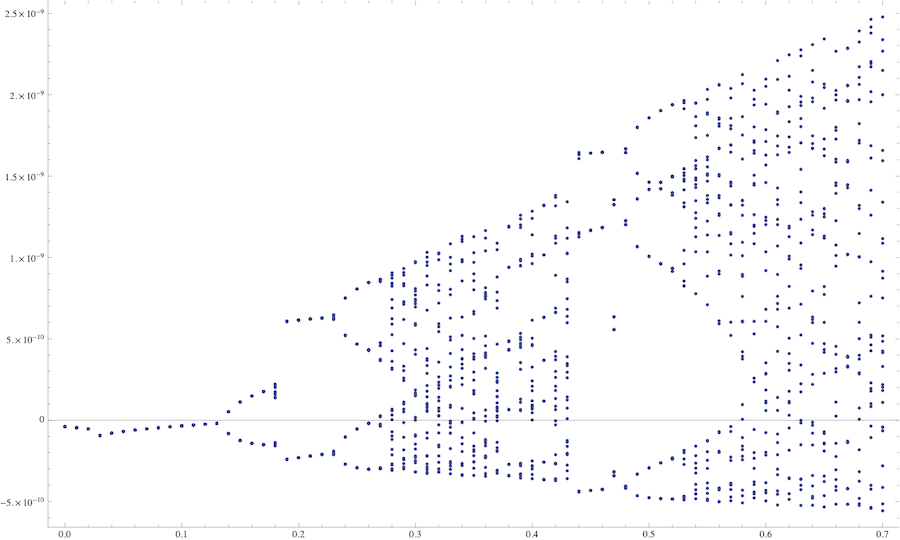
\includegraphics{simulations/circuit.png}
		\caption{Simulation Bifurcation Diagram}
		\label{fig: Simulation Bifurcation Diagram}
	\end{figure}

	\begin{figure}
		\centering
		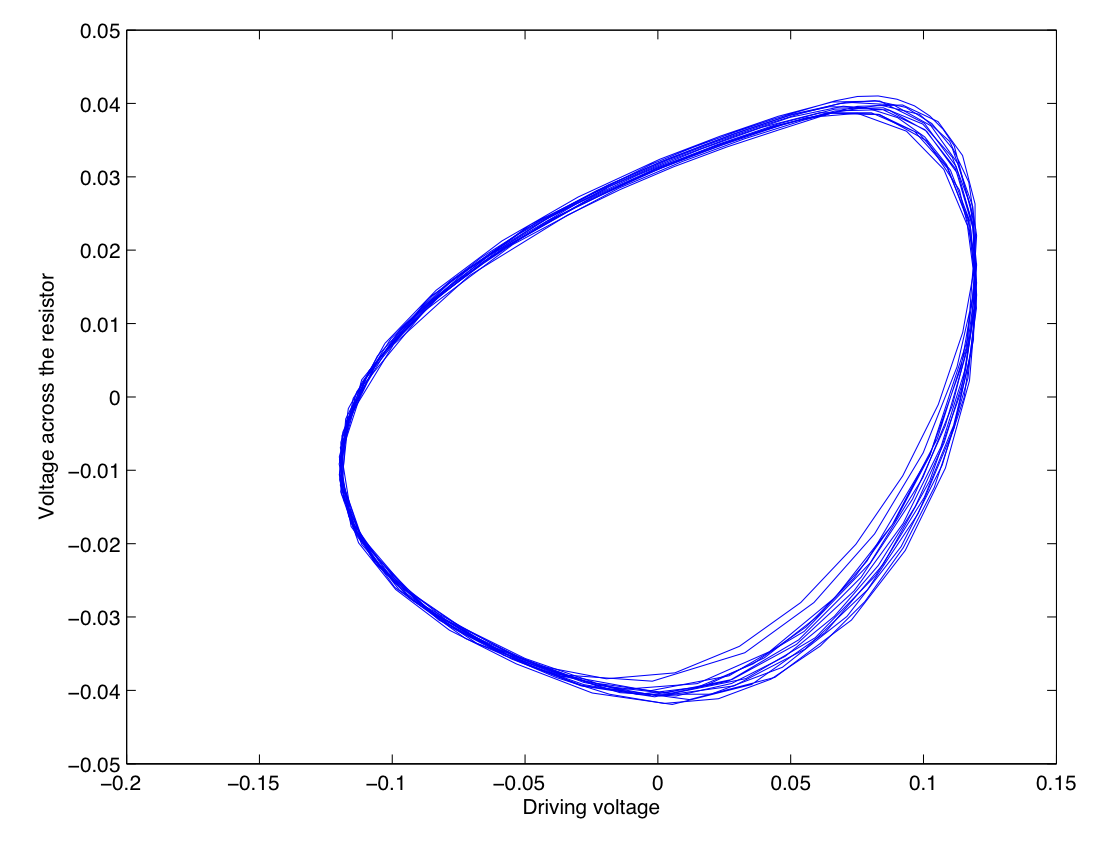
\includegraphics{simulations/plotnu0120.png}
		\caption{Simulation with $\nu=0.120$}
		\label{fig:sim.0120}
	\end{figure}
	
	\begin{figure}
		\centering
		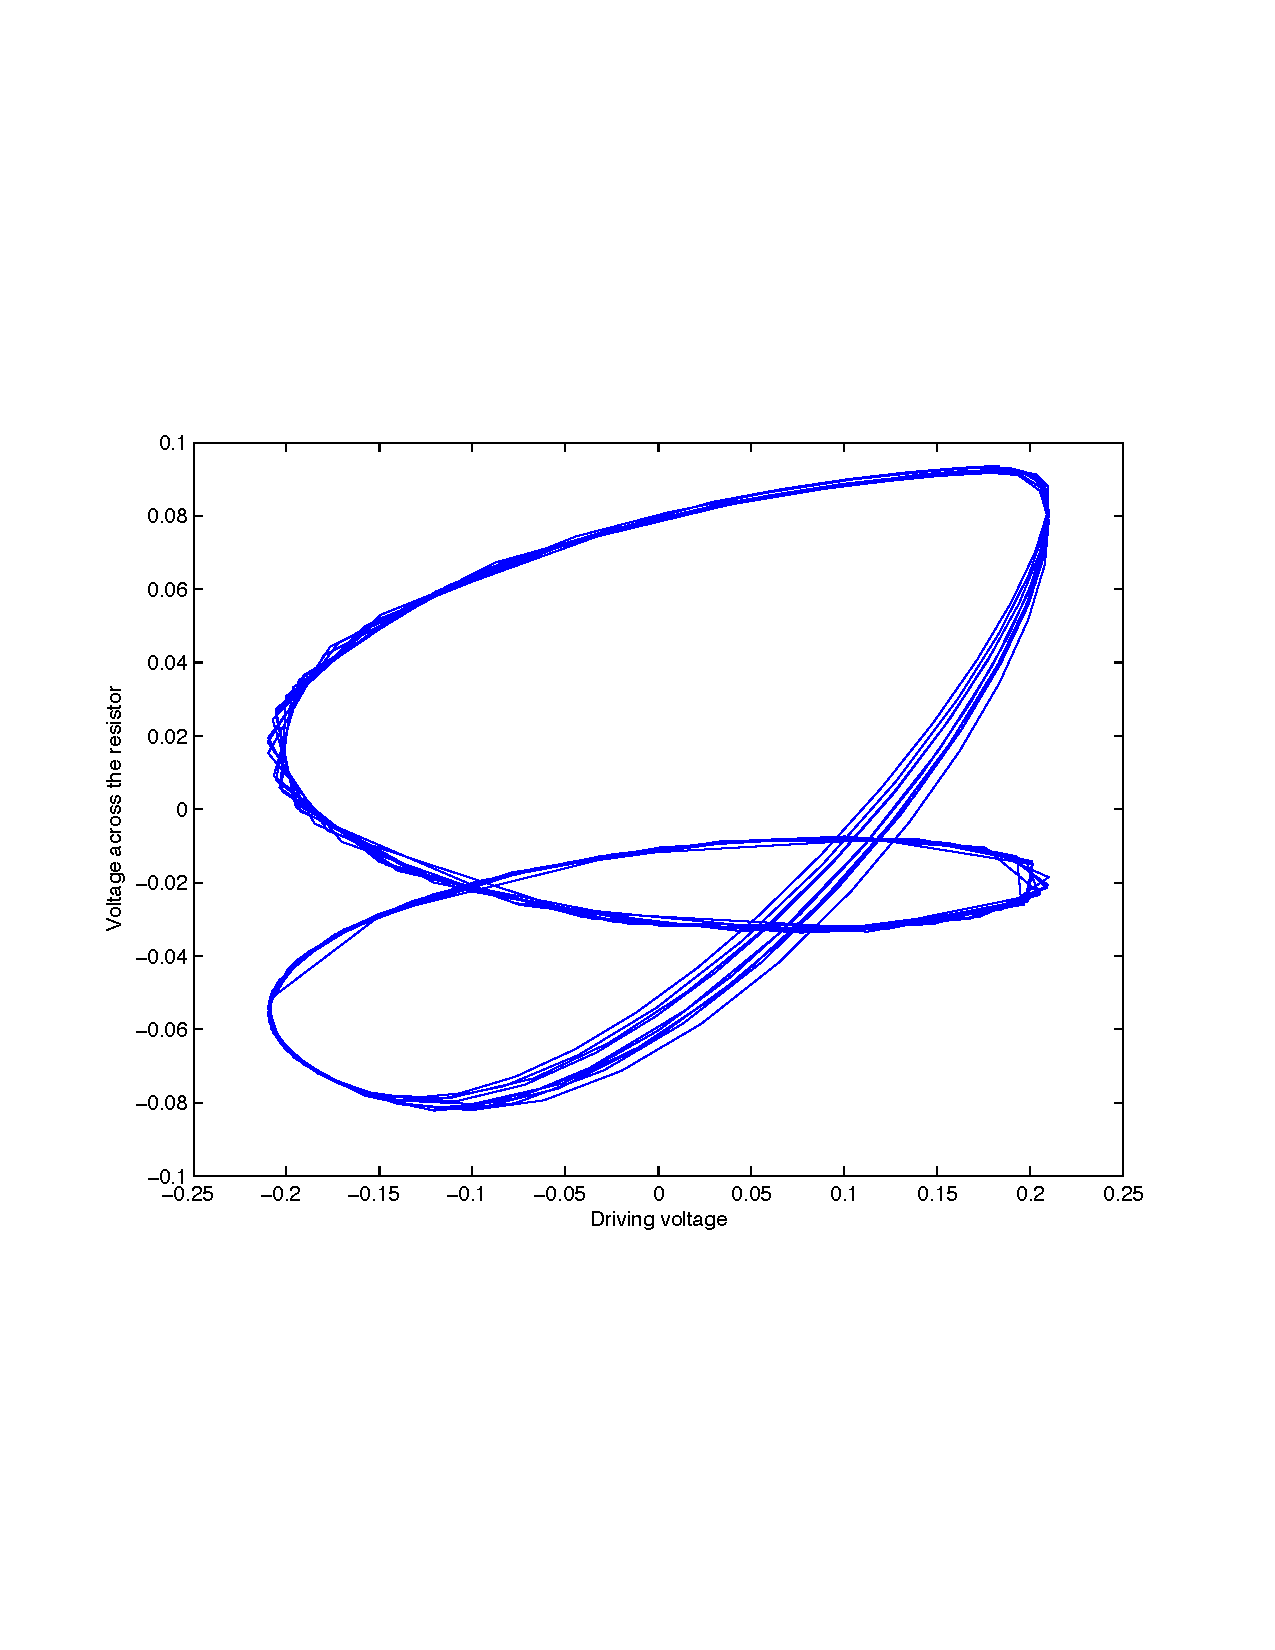
\includegraphics{simulations/plot0210.pdf}
		\caption{Simulation with $\nu=0.210$}
		\label{fig:sim.0210}
	\end{figure}

	\begin{figure}
		\centering
		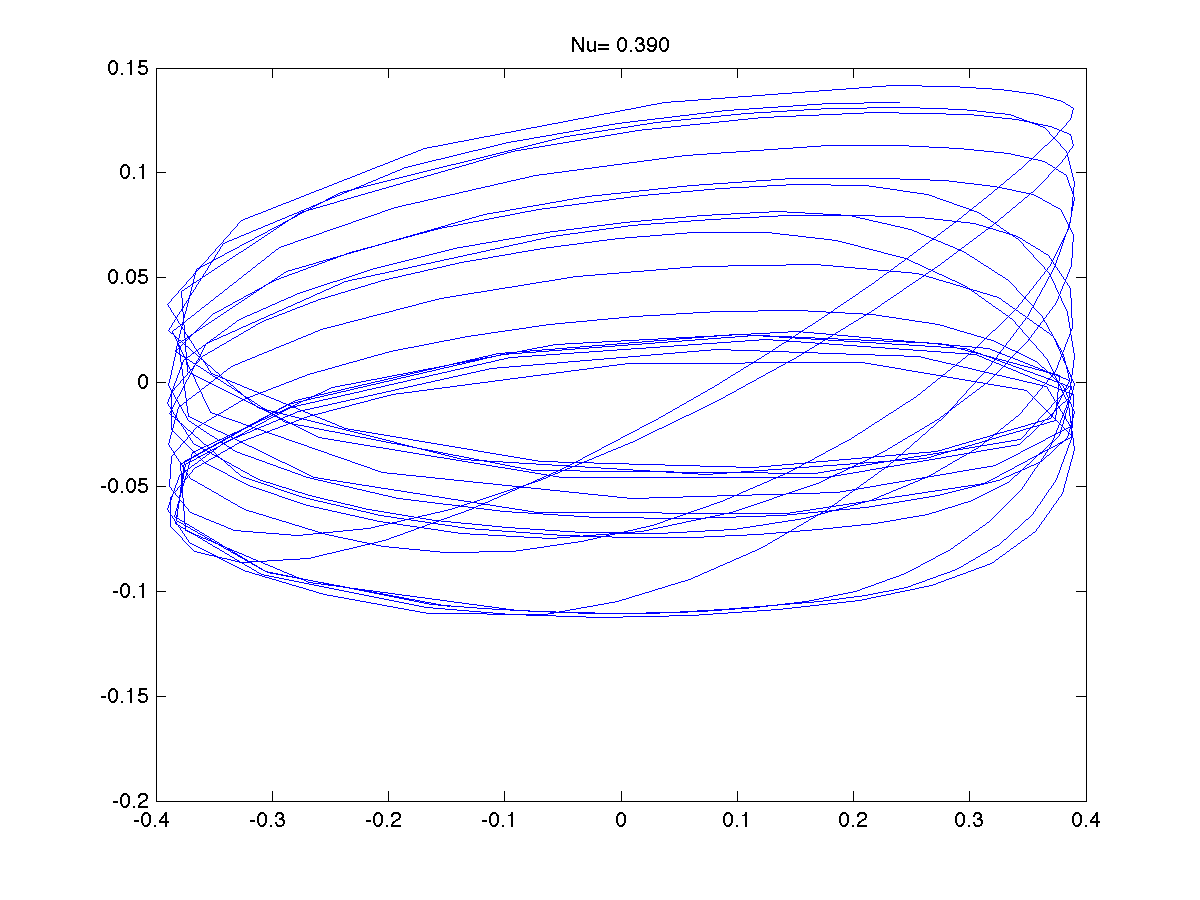
\includegraphics{simulations/plotnu0390.png}
		\caption{Chaos at $\nu=0.390$}
		\label{fig:sim.0390}
	\end{figure}

	\begin{figure}
		\centering
		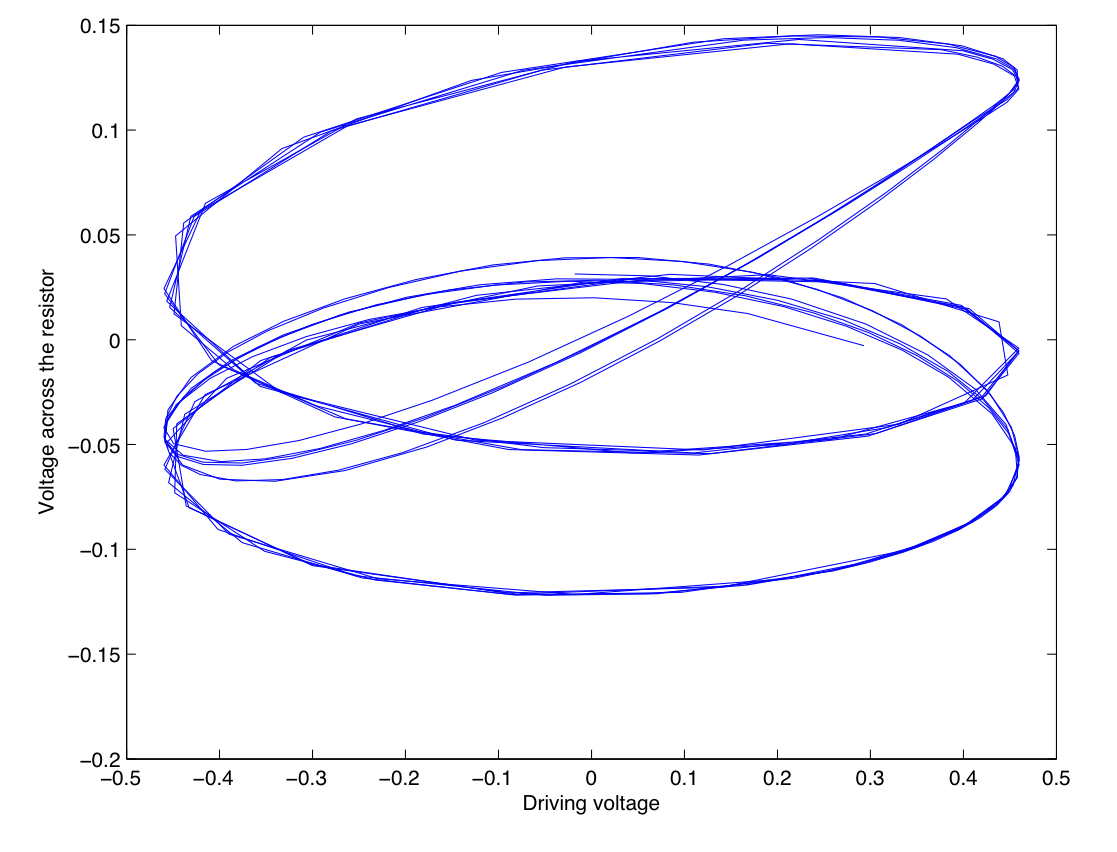
\includegraphics{simulations/plotnu0460.png}
		\caption{Simulation at $\nu=0.460$}
		\label{fig:sim.0460}
	\end{figure}

% section Simulations (end)

    %\pagebreak

\chapter*{Appendix}

\section{Data}
\label{sec:Data}

	\begin{table}[h]
		\centering
		\begin{tabular}{|l|l|l||l|l|l|}
			\hline
			Vdrive (V) & Vdrive error & Vresistor (mV)   \\ \hline
12.5 & 0.1 & 63.5                            \\ \hline
13.3 & 0.1 & 68                              \\ \hline
13.6 & 0.1 & 70                              \\ \hline
14.2 & 0.1 & 72                              \\ \hline
14.6 & 0.1 & 74                              \\ \hline
15.3 & 0.1 & 77                              \\ \hline
16.1 & 0.1 & 80.5                            \\ \hline
17.1 & 0.1 & 84                              \\ \hline
17.3 & 0.1 & 84.5                            \\ \hline
17.5 & 0.1 & 87.5                            \\ \hline
17.5 &  & 82.5                               \\ \hline
17.8 & 0.1 & 89.5                            \\ \hline
17.8 &  & 81                                 \\ \hline
18.1 & 0.1 & 92.5                            \\ \hline
18.1 &  & 77                                 \\ \hline
18.5 & 0.1 & 94                              \\ \hline
18.5 &  & 75                                 \\ \hline
18.9 & 0.1 & 96.5                            \\ \hline
18.9 &  & 73                                 \\ \hline
19.3 & 0.1 & 100                             \\ \hline
19.3 &  & 70.5                               \\ \hline
19.9 & 0.1 & 105.5                           \\ \hline
19.9 &  & 69.5                               \\ \hline
20.7 & 0.1 & 71.5                            \\ \hline
20.7 &  & 112                                \\ \hline
21.1 & 0.1 & 115                             \\ \hline
21.1 &  & 72.5                               \\ \hline
21.2 & 0.1 & 117                             \\ \hline
21.2 &  & 114                                \\ \hline
21.2 &  & 76.5                               \\ \hline
21.2 &  & 70.5                               \\ \hline
21.3 & 0.1 & 119                             \\ \hline
21.3 &  & 112.5                              \\ \hline
21.3 &  & 73                                 \\ \hline
21.3 &  & 75                                 \\ \hline
21.4 & 0.1 & 120.5                           \\ \hline
21.4 &  & 112                                \\ \hline
21.4 &  & 77.5                               \\ \hline
21.4 &  & 73.5                               \\ \hline
21.5 & 0.1 & 121                             \\ \hline
21.5 &  & 112                                \\ \hline
21.5 &  & 74                                 \\ \hline
21.5 &  & 79                                 \\ \hline
21.6 & 0.1 & 122                             \\ \hline
21.6 &  & 120.5                              \\ \hline
21.6 &  & 114.5                              \\ \hline
21.6 &  & 112                                \\ \hline
21.6 &  & 80                                 \\ \hline
21.6 &  & 79                                 \\ \hline
21.6 &  & 73                                 \\ \hline
21.6 &  & 73.5                               \\ \hline
21.7 &  & CHAOS                              \\ \hline
22.3 & 0.1 & 76.5                            \\ \hline
22.3 &  & 81                                 \\ \hline
22.3 &  & 137                                \\ \hline
22.5 & 0.1 & 77.5                            \\ \hline
22.5 &  & 81.5                               \\ \hline
22.5 &  & 140                                \\ \hline
22.6 & 0.1 & 82.5                            \\ \hline
22.6 &  & 72.5                               \\ \hline
22.6 &  & 81                                 \\ \hline
22.6 &  & 83.5                               \\ \hline
22.6 &  & 141                                \\ \hline
22.6 &  & 138                                \\ \hline
22.7 & 0.1 & CHAOS                           \\ \hline
 
		\end{tabular}
		\caption{Data for Bifurcation plot, 80 kHz}
		\label{tab:80khz}
	\end{table}

	\begin{table}[h]
		\centering
		\begin{tabular}{|l|l|l|l||l|l|l|l|}
			\hline
			V$_{\rm drive}$ (V) & $\sigma_{\rm V_{\rm drive}}$ & V$_{\rm R}$ (mV) & $\sigma_{\rm V_{\rm R}}$ &V$_{\rm drive}$ (V) & $\sigma_{\rm V_{\rm drive}}$ & V$_{\rm R}$ (mV) & $\sigma_{\rm V_{\rm R}}$       \\ \hline
14.5 & 0.1 & 55.5 & 5                                     &  20.8 & 0.1 & 92.5 &                                    \\ \hline
14.9 & 0.1 & 58 & 5                                       &  20.8 &  & 86.5 &                                       \\ \hline
15.3 & 0.1 & 59 & 5                                       &  20.8 &  & 57 &                                         \\ \hline
15.7 & 0.1 & 61.5 & 5                                     &  20.8 &  & 61 &                                         \\ \hline
15.7 &  & 57 &                                            &  21.1 & 0.1 & 93 &                                      \\ \hline
16.1 & 0.1 & 64.5 &                                       &  21.1 &  & 91.5 &                                       \\ \hline
16.1 &  & 55 &                                            &  21.1 &  & 88.5 &                                       \\ \hline
16.7 & 0.1 & 68.5 &                                       &  21.1 &  & 85.5 &                                       \\ \hline
16.7 &  & 52.5 &                                          &  21.1 &  & 64 &                                         \\ \hline
17.1 & 0.1 & 71 &                                         &  21.1 &  & 61 &                                         \\ \hline
17.1 &  & 51.5 &                                          &  21.1 &  & 56.5 &                                       \\ \hline
17.5 & 0.1 & 73.5 &                                       &  21.1 &  & 55.5 &                                       \\ \hline
17.5 &  & 50.5 &                                          &  21.2 &  & CHAOS &                                      \\ \hline
18.1 & 0.1 & 77 &                                         &  22.1 & 0.1 & 61 &                                      \\ \hline
18.1 &  & 50.5 &                                          &  22.1 &  & 76.5 &                                       \\ \hline
18.7 & 0.1 & 50.5 &                                       &  22.1 &  & 95 &                                         \\ \hline
18.7 &  & 80 &                                            &  22.3 & 0.1 & 110 &                                     \\ \hline
19.5 & 0.1 & 85.5 &                                       &  22.3 &  & 108.5 &                                      \\ \hline
19.5 &  & 54 &                                            &  22.3 &  & 64 &                                         \\ \hline
19.9 & 0.1 & 86.5 &                                       &  22.3 &  & 66 &                                         \\ \hline
19.9 &  & 54.5 &                                          &  22.3 &  & 65 &                                         \\ \hline
20.3 & 0.1 & 88.5 &                                       &  22.3 &  & 57 &                                         \\ \hline
20.3 &  & 86 &                                            &  22.5 &  & CHAOS &                                      \\ \hline
20.3 &  & 54 &                                                                                                      \\ \cline{1-4}
20.3 &  & 55.5 &                                                                                                    \\ \cline{1-4}
20.5 & 0.1 & 90 &                                                                                                   \\ \cline{1-4}
20.5 &  & 86.5 &                                                                                                    \\ \cline{1-4}
20.5 &  & 59 &                                                                                                      \\ \cline{1-4}
20.5 &  & 54.5 &                                                                                                    \\ \cline{1-4}
                                  
                                  
                                  
                                  
                                  
                                  
                                  
                                  
                                  
                                  
                                  
                                  
                                  
                                  
                                  
                                  
                                  
                                  
                                  
                                  
                                  
                                  
                                  
 
		\end{tabular}
		\caption{Data for Bifurcation plot, 100 kHz}
		\label{tab:100khz}
	\end{table}

	\begin{table}[h]
		\centering
		\begin{tabular}{|c|c|c|c|c|}
			\hline
			V$_{\rm drive}$ (mV) & Frequency (kHz) & Freq. error & $\delta$ & $\sigma_{\delta}$   \\ \hline
10443.97 & 24.15 & 0.22 & 4.96 & 1.88              \\ \hline
 & 38.38 & 0.69 &  &                                                \\ \hline
 & 41.25 & 0.70 &  &                                                 \\ \hline
 & 24.14 & 0.22 & 4.28 & 1.45                         \\ \hline
 & 38.06 & 0.69 &  &                                                \\ \hline
 & 41.31 & 0.70 &  &                                                 \\ \hline
 & 24.13 & 0.22 & 4.82 & 1.80                         \\ \hline
 & 38.19 & 0.69 &  &                                                \\ \hline
 & 41.11 & 0.70 &  &                                                 \\ \hline
 & 24.07 & 0.22 & 4.73 & 1.73                         \\ \hline
 & 38.16 & 0.69 &  &                                                \\ \hline
 & 41.14 & 0.70 &  &                                                 \\ \hline
 & 24.15 & 0.22 & 4.54 & 1.62                         \\ \hline
 & 38.08 & 0.69 &  &                                                \\ \hline
 & 41.15 & 0.70 &  &                                                 \\ \hline
 
		\end{tabular}
		\caption{Five trials at 10.4 V. Frequency varied.}
		\label{tab:chaos3}
	\end{table}

	\begin{table}[h] 
		\centering
		\begin{tabular}{|l|l|l|l|l|l|l|l|l|l|l|l|}
			\hline
			$\nu$ (kHz) & $\nu$ err & $V_{D}$ (mV) & $V_{D}$ err & $V_{R}$ (mV) & $V_{R}$ err & $\Delta V_{R}$ & $\Delta V_{R}$ err & $\delta$ & $\delta$ err & $\alpha$ & $\alpha$ err    \\ \hline
80 & 0.1 & 7884.2 & 23.8 & 89.0 & 6.0 &  &  & 4.7 & 1.3 & 4.7 & 9.8                                                           \\ \hline
 &  & 9348.0 & 46.0 & 117.5 & 7.0 & 44.5 & 9.9 & 5.9 & 9.6 & 6.4 & 17.6                                             \\ \hline
 &  &  &  & 73 &  &  &  &  &  & $\infty$ & $\infty$                                                                                                                   \\ \hline
 &  & 9656.3 & 59.6 & 123.0 & 7.0 & 9.5 & 9.9 &  &  & 8.8 & 29.0                                                                      \\ \hline
 &  &  &  & 113.5 &  &  &  &  &  &  &                                                                                                                                \\ \hline
 &  &  &  & 79.5 &  & 5.0 &  &  &  &  &                                                                                                                                \\ \hline
 &  &  &  & 74.5 &  &  &  &  &  &  &                                                                                                                                 \\ \hline
 &  & 9708.6 & 49.3 & 124.5 & 7.0 & 2.0 & 9.9 &  &  &  &                                                                                               \\ \hline
 &  &  &  & 122.5 &  &  &  &  &  &  &                                                                                                                                \\ \hline
 &  &  &  & 116.0 &  & 4.0 &  &  &  &  &                                                                                                                                 \\ \hline
 &  &  &  & 112.0 &  &  &  &  &  &  &                                                                                                                                  \\ \hline
 &  &  &  & 83.5 &  & 5.0 &  &  &  &  &                                                                                                                                \\ \hline
 &  &  &  & 78.5 &  &  &  &  &  &  &                                                                                                                                 \\ \hline
 &  &  &  & 75.0 &  & 0.5 &  &  &  &  &                                                                                                                                \\ \hline
 &  &  &  & 75.5 &  &  &  &  &  &  &                                                                                                                                 \\ \hline\hline
79.6 & 0.1 & 7854.5 & 22.8 & 87.0 & 6.0 &  &  & 4.8 & 1.3 & 4.5 & 9.4                                                        \\ \hline
 &  & 9316.8 & 45.0 & 117.0 & 7.0 & 43.0 & 9.9 & 4.3 & 5.5 & 6.1 & 16.9                                                        \\ \hline
 &  &  &  & 74.0 &  &  &  &  &  & $\infty$ & $\infty$                                                                                                                    \\ \hline
 &  & 9623.7 & 60.6 & 123.0 & 7.0 & 9.5 & 9.9 &  &  & 8.4 & 28.0                                                                      \\ \hline
 &  &  &  & 113.5 &  &  &  &  &  &  &                                                                                                                                \\ \hline
 &  &  &  & 80.0 &  & 5.0 &  &  &  &  &                                                                                                                                  \\ \hline
 &  &  &  & 75.0 &  &  &  &  &  &  &                                                                                                                                   \\ \hline
 &  & 9694.4 & 48.3 & 125.0 & 7.0 & 2.0 & 9.9 &  &  &  &                                                                                                  \\ \hline
 &  &  &  & 123.0 &  &  &  &  &  &  &                                                                                                                                  \\ \hline
 &  &  &  & 116.5 &  & 4.0 &  &  &  &  &                                                                                                                               \\ \hline
 &  &  &  & 112.5 &  &  &  &  &  &  &                                                                                                                                \\ \hline
 &  &  &  & 84.0 &  & 5.0 &  &  &  &  &                                                                                                                                  \\ \hline
 &  &  &  & 79 &  &  &  &  &  &  &                                                                                                                                   \\ \hline
 &  &  &  & 75 &  & 0.5 &  &  &  &  &                                                                                                                                \\ \hline
 &  &  &  & 75.5 &  &  &  &  &  &  &                                                                                                                                 \\ \hline\hline
80 & 0.1 & 7856.0 & 21.8 & 87.0 & 6.0 &  &  & 4.9 & 1.4 & 4.4 & 9.3                                                                  \\ \hline
 &  & 9321.1 & 45.0 & 117.0 & 7.0 & 42.5 & 9.9 & 5.1 & 7.7 & 4.7 & 10.6                                                 \\ \hline
 &  &  &  & 74.5 &  &  &  &  &  & 36.5 & 518.1                                                                                                                 \\ \hline
 &  & 9618.1 & 60.6 & 123.0 & 7.0 & 9.5 & 9.9 &  &  & 6.6 & 18.3                                                                      \\ \hline
 &  &  &  & 113.5 &  &  &  &  &  &  &                                                                                                                                \\ \hline
 &  &  &  & 81.0 &  & 6.0 &  &  &  &  &                                                                                                                                  \\ \hline
 &  &  &  & 75.0 &  &  &  &  &  &  &                                                                                                                                   \\ \hline
 &  & 9676.0 & 48.3 & 124.0 & 7.0 & 2 & 9.9 &  &  &  &                                                                                                 \\ \hline
 &  &  &  & 122.0 &  &  &  &  &  &  &                                                                                                                                  \\ \hline
 &  &  &  & 115.0 &  & 2.5 &  &  &  &  &                                                                                                                               \\ \hline
 &  &  &  & 112.5 &  &  &  &  &  &  &                                                                                                                                \\ \hline
 &  &  &  & 83.5 &  & 5.0 &  &  &  &  &                                                                                                                                \\ \hline
 &  &  &  & 78.5 &  &  &  &  &  &  &                                                                                                                                 \\ \hline
 &  &  &  & 75.0 &  & 0.5 &  &  &  &  &                                                                                                                                \\ \hline
 &  &  &  & 74.5 &  &  &  &  &  &  &                                                                                                                                 \\ \hline\hline
80 & 0.1 & 7831.9 & 22.8 & 86.5 & 6.0 &  &  & 4.9 & 1.3 & 6.8 & 20.6                                                                \\ \hline
 &  & 9305.5 & 46.0 & 116.0 & 7.0 & 42.0 & 9.9 & 6.2 & 10.9 & 7.6 & 25.2                                                  \\ \hline
 &  &  &  & 74.0 &  &  &  &  &  & 19.0 & 136.6                                                                                                                     \\ \hline
 &  & 9603.9 & 59.6 & 121.5 & 7.0 & 8.0 & 9.9 &  &  & 10.9 & 45.6                                                                      \\ \hline
 &  &  &  & 113.5 &  &  &  &  &  &  &                                                                                                                                \\ \hline
 &  &  &  & 79.0 &  & 4.0 &  &  &  &  &                                                                                                                                  \\ \hline
 &  &  &  & 75.0 &  &  &  &  &  &  &                                                                                                                                   \\ \hline
 &  & 9652.0 & 48.3 & 123.5 & 7.0 & 3.0 & 9.9 &  &  &  &                                                                                               \\ \hline
 &  &  &  & 120.5 &  &  &  &  &  &  &                                                                                                                                \\ \hline
 &  &  &  & 115.5 &  & 3.5 &  &  &  &  &                                                                                                                             \\ \hline
 &  &  &  & 112.0 &  &  &  &  &  &  &                                                                                                                                  \\ \hline
 &  &  &  & 83.0 &  & 2.0 &  &  &  &  &                                                                                                                                  \\ \hline
 &  &  &  & 81.0 &  &  &  &  &  &  &                                                                                                                                   \\ \hline
 &  &  &  & 74.5 &  & 0.5 &  &  &  &  &                                                                                                                              \\ \hline
 &  &  &  & 75.0 &  &  &  &  &  &  &                                                                                                                                   \\ \hline
 &  &  &  &  &  &  &  &  &  &  &                                                                                                                                     \\ \hline
80 & 0.1 & 7823.4 & 21.8 & 86.5 & 6.0 &  &  & 4.9 & 1.3 & 4.7 & 10.6                                                        \\ \hline
 &  & 9285.7 & 44.0 & 115.5 & 7.0 & 42.5 & 9.9 & 3.8 & 4.4 & 5.1 & 12.2                                                     \\ \hline
 &  &  &  & 73.0 &  &  &  &  &  & 37.5 & 532.1                                                                                                                    \\ \hline
 &  & 9581.3 & 59.6 & 121.5 & 7.0 & 9.5 & 9.9 &  &  & 9.4 & 34.7                                                                          \\ \hline
 &  &  &  & 112.0 &  &  &  &  &  &  &                                                                                                                                  \\ \hline
 &  &  &  & 79.0 &  & 5.0 &  &  &  &  &                                                                                                                                  \\ \hline
 &  &  &  & 74.0 &  &  &  &  &  &  &                                                                                                                                   \\ \hline
 &  & 9659.1 & 49.3 & 123.0 & 7.0 & 2.5 & 9.9 &  &  &  &                                                                                               \\ \hline
 &  &  &  & 120.5 &  &  &  &  &  &  &                                                                                                                                \\ \hline
 &  &  &  & 114.5 &  & 3.0 &  &  &  &  &                                                                                                                               \\ \hline
 &  &  &  & 111.5 &  &  &  &  &  &  &                                                                                                                                \\ \hline
 &  &  &  & 83.5 &  & 4.0 &  &  &  &  &                                                                                                                                \\ \hline
 &  &  &  & 79.5 &  &  &  &  &  &  &                                                                                                                                 \\ \hline
 &  &  &  & 74.0 &  & 1.0 &  &  &  &  &                                                                                                                                  \\ \hline
 &  &  &  & 75.0 &  &  &  &  &  &  &                                                                                                                                   \\ \hline
 &  &  &  &  &  &  &  &  &  &  &                                                                                                                                     \\ \hline
  
		\end{tabular}
		\caption{Five trials at 80 kHz. Voltage varied.}
		\label{tab:chaos2}
	\end{table}
	
	\begin{table}[h]
		\centering
		\begin{tabular}{|l|l|l|l|l|l|l|l|l|l|l|l|}
			\hline
			$\nu$ (kHz) & $V_{D}$ (mV) & $V_{R}$ (mV) & $\Delta V_{R}$ & $\delta$ & $\alpha$    \\ \hline
$120.0 \pm 0.1$ & $6040.1 \pm 37.4$ & $48.0 \pm 7.0$ & & $4.0 \pm 0.5$ & $6.5 \pm 26.2$                                                         \\ \hline
 &  $8554.6 \pm 44.4$ & $71.0 \pm 6.0$ & $25.8 \pm 8.5$ & $7.9 \pm 10.9$ & $7.7 \pm 36.1$                                               \\ \hline
 &  & 45.3 &  &  & $29.7 \pm 482.9$                                                                                                         \\ \hline
 & $9189.6 \pm 60.0$ & $75.3 \pm 6.0$ & $4.5 \pm 8.5$ &  & $7.4 \pm 31.9$                                                                    \\ \hline
 &  & 70.8 &  &  &  &                                                                                                                                \\ \hline
 &  & 50.3 & 3.5 &  &  &                                                                                                                             \\ \hline
 &  & 46.8 &  &  &  &                                                                                                                                \\ \hline
 &  $9270.2 \pm 88.3$ & $76.0 \pm 6.0$ & $1.3 \pm 8.5$ &  &  &                                                                                              \\ \hline
 &  & 74.8 &  &  &  &                                                                                                                                \\ \hline
 &  & 72.0 & 1.8 &  &  &                                                                                                                               \\ \hline
 &  &  70.5 &  &  &  &                                                                                                                                \\ \hline
 &  &  52.0 &  2.8 &  &  &                                                                                                                               \\ \hline
 &  &  49.3 &  &  &  &                                                                                                                                \\ \hline
 &  &  47.0 & 0.5 &  &  &                                                                                                                                \\ \hline
 &  &  47.5 &  &  &  &                                                                                                                                 \\ \hline
 &  &  &  &  &  &                                                                                                                                     \\ \hline
120.0 & 0.1 & 6055.7 & 37.4 & 48.0 & 7.0 &  &  & 4.0 & 0.5 & 7.9 & 36.9                                                          \\ \hline
 &  & 8563.1 & 44.4 & 71.3 & 6.0 & 26.0 & 8.5 & 5.3 & 5.1 & 14.5 & 120.2                                                       \\ \hline
 &  &  &  & 45.3 &  &  &  &  &  & 22.3 & 273.2                                                                                                               \\ \hline
 &  & 9189.6 & 60.0 & 75.0 & 6.0 & 4.3 & 8.5 &  &  & 6.8 & 27.3                                                                      \\ \hline
 &  &  &  & 70.8 &  &  &  &  &  &  &                                                                                                                                \\ \hline
 &  &  &  & 50.5 &  & 3.8 &  &  &  &  &                                                                                                                             \\ \hline
 &  &  &  & 46.8 &  &  &  &  &  &  &                                                                                                                                \\ \hline
 &  & 9308.4 & 88.3 & 76.5 & 6.0 & 1.5 & 8.5 &  &  &  &                                                                                             \\ \hline
 &  &  &  & 75.0 &  &  &  &  &  &  &                                                                                                                                   \\ \hline
 &  &  &  & 72.5 &  & 2.8 &  &  &  &  &                                                                                                                             \\ \hline
 &  &  &  & 69.8 &  &  &  &  &  &  &                                                                                                                                \\ \hline
 &  &  &  & 52.5 &  & 2.8 &  &  &  &  &                                                                                                                             \\ \hline
 &  &  &  & 49.8 &  &  &  &  &  &  &                                                                                                                                \\ \hline
 &  &  &  & 47.0 &  & 0.5 &  &  &  &  &                                                                                                                                \\ \hline
 &  &  &  & 47.5 &  &  &  &  &  &  &                                                                                                                                 \\ \hline
 &  &  &  &  &  &  &  &  &  &  &                                                                                                                                     \\ \hline
120.0 & 0.1 & 6050.0 & 37.4 & 48.0 & 7.0 &  &  & 3.8 & 0.5 & 4.9 & 15.4                                                          \\ \hline
 &  & 8554.6 & 44.4 & 70.8 & 6.0 & 25.5 & 8.5 & 8.2 & 11.3 & 6.9 & 29.9                                              \\ \hline
 &  &  &  & 45.3 &  &  &  &  &  & 44.0 & 1068.2                                                                                                                  \\ \hline
 &  & 9213.6 & 60.0 & 75.3 & 6 & 4.8 & 8.5 &  &  & 7.3 & 31.5                                                                   \\ \hline
 &  &  &  & 70.5 &  &  &  &  &  &  &                                                                                                                                 \\ \hline
 &  &  &  & 50.5 &  & 3.5 &  &  &  &  &                                                                                                                              \\ \hline
 &  &  &  & 47.0 &  &  &  &  &  &  &                                                                                                                                   \\ \hline
 &  & 9294.2 & 88.3 & 75.5 & 6.0 & 0.5 & 8.5 &  &  &  &                                                                                             \\ \hline
 &  &  &  & 75.0 &  &  &  &  &  &  &                                                                                                                                   \\ \hline
 &  &  &  & 72.0 &  & 1.8 &  &  &  &  &                                                                                                                               \\ \hline
 &  &  &  & 70.3 &  &  &  &  &  &  &                                                                                                                                \\ \hline
 &  &  &  & 52.5 &  & 3.0 &  &  &  &  &                                                                                                                                \\ \hline
 &  &  &  & 49.5 &  &  &  &  &  &  &                                                                                                                                 \\ \hline
 &  &  &  & 47.5 &  & 0.5 &  &  &  &  &                                                                                                                              \\ \hline
 &  &  &  & 48.0 &  &  &  &  &  &  &                                                                                                                                   \\ \hline
 &  &  &  &  &  &  &  &  &  &  &                                                                                                                                     \\ \hline
120.0 & 0.1 & 6051.4 & 37.4 & 48.3 & 7.0 &  &  & 4.1 & 0.6 & 6.6 & 26.5                                                      \\ \hline
 &  & 8556.0 & 44.4 & 70.8 & 6.0 & 25.5 & 8.5 & 4.1 & 3.3 & 10.8 & 67.7                                                   \\ \hline
 &  &  &  & 45.3 &  &  &  &  &  & 12.7 & 90.8                                                                                                         \\ \hline
 &  & 9161.3 & 61.0 & 74.8 & 6.0 & 4.0 & 8.5 &  &  & 8.1 & 37.7                                                                      \\ \hline
 &  &  &  & 70.8 &  &  &  &  &  &  &                                                                                                                                \\ \hline
 &  &  &  & 46.8 &  & 3.3 &  &  &  &  &                                                                                                                            \\ \hline
 &  &  &  & 50.0 &  &  &  &  &  &  &                                                                                                                                   \\ \hline
 &  & 9308.4 & 89.3 & 75.5 & 6.0 & 0.8 & 8.5 &  &  &  &                                                                                            \\ \hline
 &  &  &  & 74.8 &  &  &  &  &  &  &                                                                                                                                \\ \hline
 &  &  &  & 72.3 &  & 2.0 &  &  &  &  &                                                                                                                               \\ \hline
 &  &  &  & 70.3 &  &  &  &  &  &  &                                                                                                                                \\ \hline
 &  &  &  & 52.5 &  & 1.5 &  &  &  &  &                                                                                                                              \\ \hline
 &  &  &  & 51.0 &  &  &  &  &  &  &                                                                                                                                   \\ \hline
 &  &  &  & 47.3 &  & 0.5 &  &  &  &  &                                                                                                                             \\ \hline
 &  &  &  & 47.8 &  &  &  &  &  &  &                                                                                                                                \\ \hline
 &  &  &  &  &  &  &  &  &  &  &                                                                                                                                     \\ \hline
120.0 & 0.1 & 6059.9 & 37.4 & 48.0 & 7.0 &  &  & 4.0 & 0.5 & 12.1 & 86.9                                                          \\ \hline
 &  & 8563.1 & 45.4 & 70.8 & 6.0 & 25.5 & 8.5 & 6.2 & 7.0 & 9.4 & 53.2                                              \\ \hline
 &  &  &  & 45.3 &  &  &  &  &  & 22.0 & 270.2                                                                                                                   \\ \hline
 &  & 9196.6 & 61.0 & 75.0 & 6.0 & 4.3 & 8.5 &  &  & 7.3 & 31.5                                                                      \\ \hline
 &  &  &  & 70.8 &  &  &  &  &  &  &                                                                                                                                \\ \hline
 &  &  &  & 50.3 &  & 3.5 &  &  &  &  &                                                                                                                             \\ \hline
 &  &  &  & 46.8 &  &  &  &  &  &  &                                                                                                                                \\ \hline
 &  & 9298.5 & 89.3 & 76.0 & 6.0 & 2.5 & 8.5 &  &  &  &                                                                                               \\ \hline
 &  &  &  & 74.8 &  &  &  &  &  &  &                                                                                                                                \\ \hline
 &  &  &  & 72.3 &  & 2.0 &  &  &  &  &                                                                                                                               \\ \hline
 &  &  &  & 70.3 &  &  &  &  &  &  &                                                                                                                                \\ \hline
 &  &  &  & 52.3 &  & 2.5 &  &  &  &  &                                                                                                                             \\ \hline
 &  &  &  & 49.8 &  &  &  &  &  &  &                                                                                                                                \\ \hline
 &  &  &  & 47.0 &  & 0.5 &  &  &  &  &                                                                                                                                \\ \hline
 &  &  &  & 47.5 &  &  &  &  &  &  &                                                                                                                                 \\ \hline
 
		\end{tabular}
		\caption{Five trials at 120 kHz. Voltage varied.}
		\label{tab:chaos2}
	\end{table}

\section{Code}
\label{sec: Code}

\begin{figure}[h]
\begin{lstlisting}
function dy = ode1(t,y)

global C1 C2 R1 L1 f E0 nu

dy = zeros(2,1);
dy(1) = y(2);
dy(2) = (-R1*y(2)-( (C2-C1)/(2*C2*C1)*abs(y(1))+ (C1+C2)/(2*C1*C2)*y(1)+E0)
	+ nu * sin(2*pi*f*t))/L1;
\end{lstlisting}
\caption{Code for RL circuit ODE}
\label{code:ode}
\end{figure}

\begin{figure}[h]
\begin{lstlisting}
global C1 C2 R1 L1 f E0 nu

C1 = 0.1 * 10^-6;
C2 = 400.0 * 10^-12;
R1 = 60.0;
L1 = 100.0 * 10^-6;
f = 700000.0;
E0 = 0.1;
nuinit = 0.1;

nuinc = 0.01;
numax = 0.7;
nu = nuinit;

for j=1:((numax-nuinit)/nuinc)
    [T,Y] = ode45(@ode1,[10^-4,100.0*10^-4],[0,0]);
    plot(nu * sin(2*pi*f*T(200:600)),Y(200:600,2)*R1)
    fi = sprintf('plots2/plot.nu.%6.3f.pdf', nu);
    print('-dpdf', fi)
    nu = nu + nuinc;
end
\end{lstlisting}
	\caption{Code for iterating through parameters of RL circuit}
	\label{code:run}
\end{figure}



% citations:
% http://reference.wolfram.com/legacy/v5_2/Demos/Notebooks/ChaoticCircuit.html


\end{document}

